\documentclass{article}
\usepackage{geometry}
\usepackage{titling}
\usepackage{amsmath}
\usepackage{graphicx}
\usepackage{hyperref}
 
\hypersetup{colorlinks=true,urlcolor=cyan,linkcolor=blue}


\title{Longitudinal-Transverse Motion Reconstruction \\ Methods and Preliminary Data}
\author{Brian Frost}
\date{March 2022}
\pretitle{\begin{center}\huge}
\posttitle{\end{center}}
\preauthor{\begin{center}\small}
\postauthor{\end{center}}
\predate{\begin{center}\footnotesize}
\postdate{\end{center}}
\setlength{\droptitle}{-40pt}

\begin{document}
\maketitle

\section{Introduction}
\par{Historically, the \textit{in vivo} study of cochlear mechanics has been limited to measurements of the basilar membrane (BM). The advent of optical coherence tomography (OCT) in the last decade has allowed for vibrometry at a depth, facilitating the study of intra-organ of Corti complex (OCC) motions. Of particular interest is the motion of the electromotile outer hair cells (OHCs), which play an important role in the amplifying vibration responses and increasing the range of sound-pressure levels (SPLs) over which hearing operates.}
\par{Several groups, ours included, have presented OCT measurements of OHC motion in the base of the sensitive gerbil cochleae. In some instances, these measurements have differed significantly from one another. In particular, groups have reported disparate phase differences between displacements in the ``OHC region" and at the BM.}
\par{Several aspects complicate these measurements. The first, and perhaps the clearest, is that the term ``OHC region" is ill-defined; the OHCs are ~40 $\mu m$ long and 10 $\mu m$ wide, and come in rows of three per longitudinal cross-section. Mechanical intuition may lead one to believe that the apical surface of the OHCs, called the Reticular lamina (RL), may move quite differently from the basal surface attached to the Deiters' cells as the OHC compresses and expands due to electromotility. It is naive to assume the entire 30$\mu m\times$40 $\mu m$ area moves uniformly.}
\par{A second complication is that measurements are taken at an angle with respect to the orientation of the cochlea, unknown \textit{a priori}. This means that (1) OCT measurements, which measure the displacement along the beam axis, measure some unknown projection of the motion; (2) measured OHC and BM may lie in different tonotopic locations.}
\par{The first of these ambiguities is discussed in some detail in the supplementary material of \href{https://www.nature.com/articles/s41467-018-05483-z}{Cooper et al, 2018}, wherein the authors discuss the hypothetical scenario where OHCs exhibit some fluid-like elliptical motion. They show modeled results under the assumption that transverse (normal to BM) OHC motion is in phase with BM motion. Their model suggested that measured OHC displacement phase could differ from transverse OHC displacement phase significantly as a function of the viewing angle, with any deviation between $-180^\text{o}$ and $+180^\text{o}$ being achievable.}
\par{The second of these ambiguities is discussed in \href{https://asa.scitation.org/doi/full/10.1121/10.0009576}{Frost et al, 2022}, wherein we developed a program which measures the relative anatomical displacements between structures in OCT measurements. We used this to account for the longitudinal displacement between OHCs and BM in a single measurement by taking a second BM measurement in the same cross-section as the first measurement's OHCs. We were able to show that this correction affected the character of the OHC phase re BM, including up to 90-degree discrepancy between displacement-accounted and unaccounted measurements at high frequencies.}
\par{With these two problems in mind, it is difficult to interpret presented OHC displacement data reported without a specified angle. The group of Ren, which uses an interferometer similar to OCT but importantly lacking imaging capabilities, has presented what they claim are purely transverse measurements of BM and OHC displacement in the base of several sensitive gerbil cochleae. Their poster at the ARO midwinter meeting of 2022 presents this most directly, but the data presented there is similar to what they have shown in Figure 1H of \href{https://elifesciences.org/articles/37625}{He et al, 2018}. While they refer to their OHC measurements as being from RL, it is difficult to assess the efficacy of this claim given their system does not image.}
\par{Here they show that RL phase leads BM sub-BF by more than 90 degrees, and that this lead decreases monotonically (with a near-linear shape) over the measured range. At about 0.8BF, the RL and BM are in phase and above this frequency RL lags BM. They also show similar results in mouse in \href{https://www.pnas.org/doi/10.1073/pnas.1607428113}{Ren et al, 2016}.}
\par{Our group's data shows a different character to OHC phase re BM. When we measure BM and OHC displacement phase in the same cross-section, as in \href{https://asa.scitation.org/doi/full/10.1121/10.0009576}{Frost et al, 2022}, we see that OHC phase leads BM across frequency. Where Ren et al see an ~80 degree lag of the OHCs re BM at high frequencies, we see a ~90 degree lead. }
\par{We have developed a method to isolate the transverse and longitudinal components of motion of structures within the OCC, focusing only on the OHC region. We account both for the relative locations of measured OHC and BM and the form of the projection onto the beam direction, while controlling for the position within the OHC region, to address the complications inherent to OCT motion measurement. In doing so, we can gain a more complete understanding of intra-OCC motions and can attempt to resolve some apparent discrepancies between different groups. In this document, I will discuss the method for acquisition of motion measurements, as well as the method for reconstruction. I will then present a preliminary data set where we have reconstructed longitudinal and transverse motion at the base of the OHC at several longitudinal locations. Finally, I will provide a short outline of my goals for future application of this program.}

\section{Methods}
\subsection{Acquisition}
\par{The acquisition process follows a few simple steps: (1) prior to acquisition, ensure the BM looks as horizontal as possible in the orienting B-Scan, (2) determine the approximate longitudinal direction and take measurements of a single structure at multiple longitudinal locations, (3) rotate the preparation and try to isolate similar cross-sections with the BM appearing horizontal in the orienting B-Scan, (4) again, find the approximate longitudinal direction and take measurements of the same structure at multiple longitudinal locations.}
\par{Ensuring that the BM appears horizontal in each cross-section ensures that the radial component of the optic axis is approximately zero. This is important, as we are attempting to simplify our problem to two dimensions -- transverse and longitudinal. Failing to account for this radial angle will make our two-dimensional reconstruction impossible.}
\par{Determining the approximate longitudinal directions works via a linear approximation of the cochlea's anatomical coordinates, similar to the planar approximation employed in \href{https://asa.scitation.org/doi/full/10.1121/10.0009576}{Frost et al, 2022}. As we only need the longitudinal direction for acquisition, this is a simpler process -- we use ThorImage and locate a landmark in some cross-section; for example, we can choose the base of the OHC, or the thickest part of the BM. We record the optical coordinates at these positions, $p_1 = (x_1,y_z,z_1)$ and $p_2 = (x_2,y_2,z_2)$. The difference between these points is a vector in the longitudinal direction, so the unit longitudinal vector is given by
	\begin{equation} \label{findl}
		l = \frac{p_2 - p_1}{|p_2-p_1|}.
	\end{equation}
We use MATLAB to list points of measurement in the longitudinal direction spaced as desired. If we start at point $q_0$, and want to measure $N$ points spaced $\delta$ apart longitudinally, then the points we measure are 
	\begin{equation}
		q_n = q_0 + n\delta l,\;n=0,1,\ldots,N-1.
	\end{equation}
}
\par{We take volume scans prior to and after each acquisition for two reasons -- (1) we can more methodically determine our longitudinal positions outside of the time constraints of an experiment, and (2) we can determine if the preparation has significantly drifted. To the effect of (2), we also take B-Scans immediately after the recordings at each position so that we can be sure of which structures we actually measured.}
\par{Figure \ref{pointselect} shows two cross-sections from a single volume where points at the same landmark have been marked with red dots. The coordinates of these points could be subtracted to give the longitudinal direction.}

\begin{figure}
	\centering
	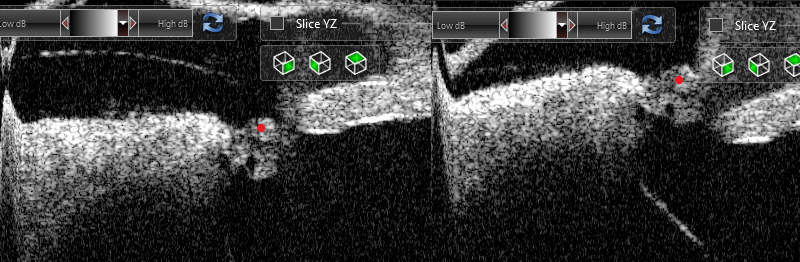
\includegraphics[width=\textwidth]{Figures/points.png}
	\caption{Two cross-sections of a volume of the base of the gerbil cochlea. Red dots show sample points on the BM at its widest position. Subtracting the coordinates of these two points would give an approximation of the longitudinal direction.}
\label{pointselect}
\end{figure}


\subsection{Registration}
\par{To reconstruct motion of a particular structure, we need to ensure that we have located the same structure at multiple angles. We have discussed a method in \href{https://asa.scitation.org/doi/full/10.1121/10.0009576}{Frost et al, 2022} for finding relative positions of points within a static volume. A two-dimensional analogue of this process allows us to find relative positions of OHC and BM in single measurements.}
\par{In our case, as we have made sure to remove the radial component of motion from our measurements, we can assume the optical ($z$) axis is comprised of only longitudinal ($l$) and transverse ($t$) components. We write the optical axis' unit vector as a two-dimensional vector in anatomical coordinates, $z = (z_l,z_t)$.}
\par{Equation \ref{findl} is used in the acquisition step to find the longitudinal vector $l$, which has optical  $x$, $y$, and $z$ components. The $z$ component of this vector represents the amount of longitudinal motion that is projected onto the optical axis, $z_l$. To find the $t$ component, we need only recall that $z$ is a unit vector so that $z_l^2 + z_t^2 = 1$. Using the notation from Equation \ref{findl}, we can write this as
	\begin{align}
		z_l &= \frac{z_2-z_1}{|p_2-p_1|}, \\
		z_t &= \sqrt{1-z_l^2}.
	\end{align}
}
\par{Knowing this, we can relate the OHC and BM longitudinal locations within a single measurement. Consider the B-Scans in Figure \ref{bscans}, in which we have selected points along a single measurement axis at both the BM and the OHC's base. We can measure the $\Delta z$ between these two points (it is simply the pixel size multiplied by the pixel difference), which tells us that the OHCs are $\Delta z \times z_l$ apical of the BM in this measurement. Having taken measurements at many longitudinal locations, we can then find a point on the BM $\Delta z \times z_l$ apical of the BM in the first measurement. These are the \textit{aligned} BM and OHC, which lie in the same longitudinal cross-section. For each set of runs at a given angle, we create a list of aligned OHC base and BM positions.}

\begin{figure}
	\centering
	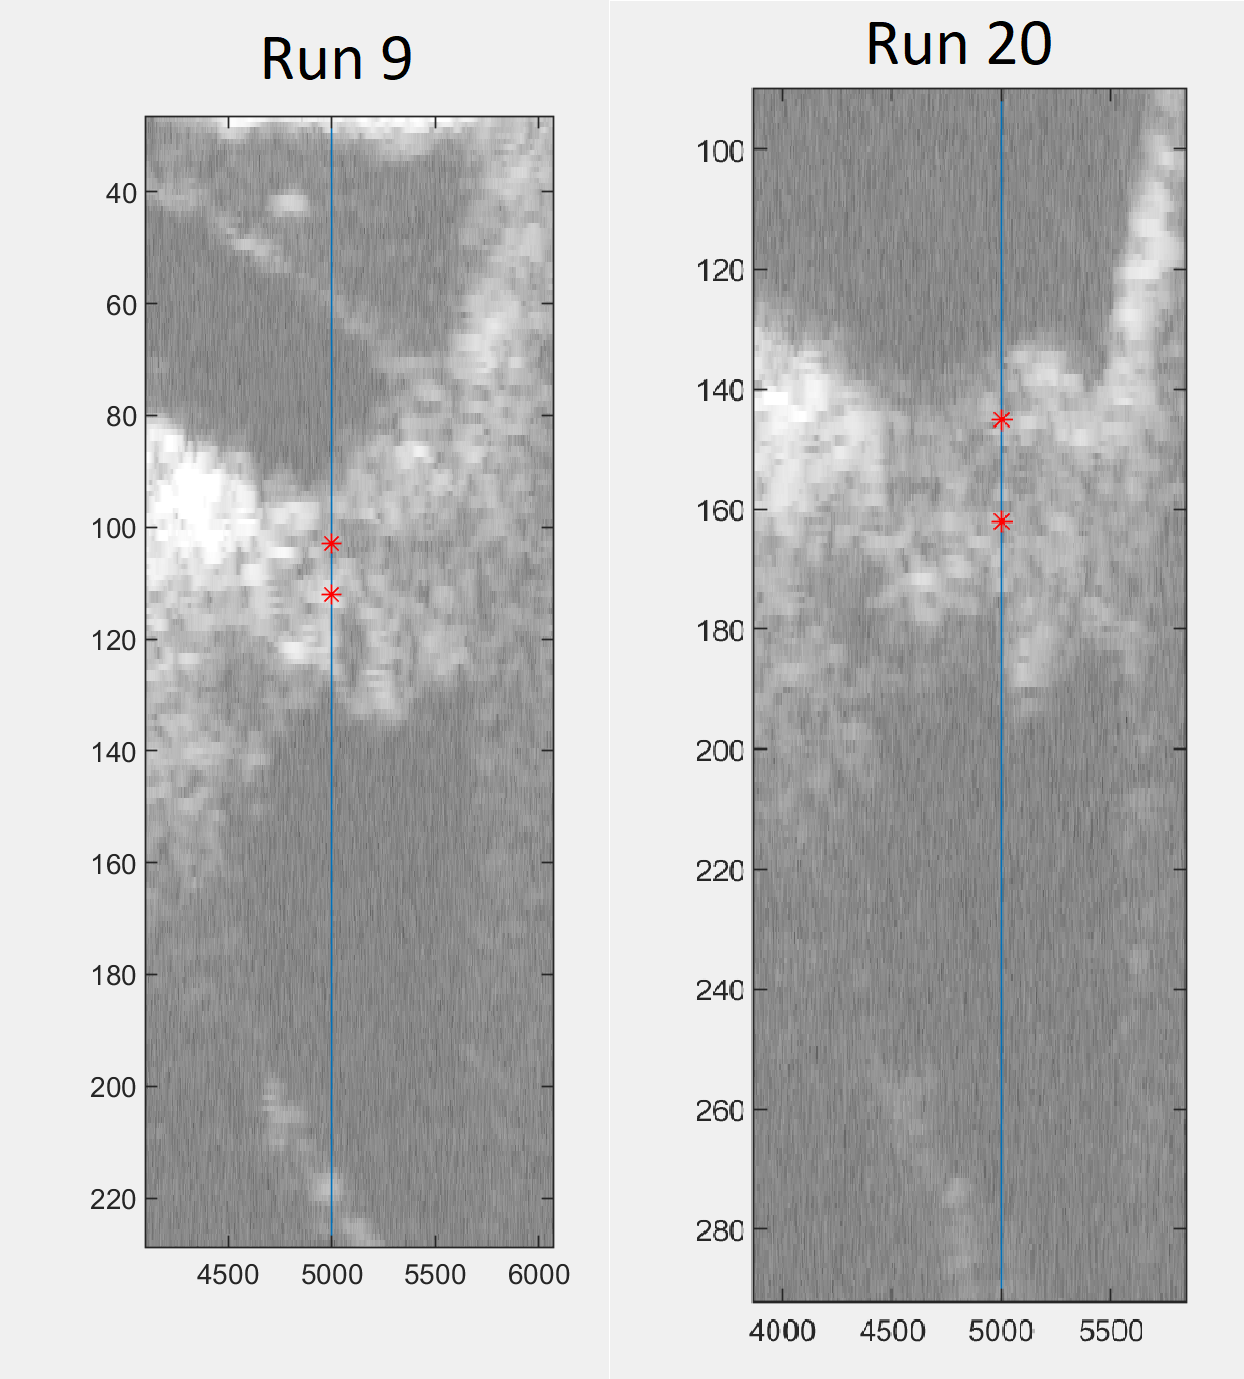
\includegraphics[width = .5\textwidth]{"Figures/BScans Points.png"}
	\caption{Two B-Scans from a single volume, taken at one angle but spaced apart by 45 $\mu$m longitudinally. On each, points marking the BM and OHC are shown. The difference between these points is used to determine the longitudinal offset between BM and OHC in the same run.}
	\label{bscans}
\end{figure}

\par{To register structures at the same locations in multiple locations, we use a method based on the phase of BM motion. It is natural to assume that the BM moves only transversely and does not vary radially, so that its phase at a specific cross-section will be identical at all measurement angles. We look for points where the measured BM phases are very close to one another at two different measurement angles. These points correspond to the same cross-section, so their \textit{aligned OHCs} also lie in the same cross-section. This is how we register OHCs measured at multiple angles.}

\subsection{Reconstruction}

\par{Each OCT measurement is a projection of a true 3-D motion onto the optical $z$ axis. In the current context, we have made efforts to eliminate the representation of radial motion in our projections, so that the problem can be framed as the projection of a 2-D longitudinal-transverse \textit{true motion} $d$ onto a 2-D transverse-longitudinal $z$ axis, forming the \textit{projected motion} $\delta$.}
\par{Above we describe the method by which we determine the $z_l$ and $z_t$ components of the optical axis in each experiment. The projection onto this axis is given by the dot product
	\begin{equation}
		\delta = z \cdot d = \begin{pmatrix}z_l& z_t\end{pmatrix}\begin{pmatrix}d_l\\d_t\end{pmatrix}.
	\end{equation}
}
\par{At each angle, if we are truly measuring at one position, $d$ will remain the same and $z$ will change. If we take measurements at two angles, we form the system of equations:
	\begin{equation}\label{projmat}
		\begin{pmatrix}\delta_1 \\ \delta_2\end{pmatrix} = \begin{pmatrix}l_1 & t_1\\l_2 & t_2\end{pmatrix}\begin{pmatrix}d_l\\d_t\end{pmatrix},
	\end{equation}
	where the rows of the matrix are the $z$ axes corresponding to each angle, and $\delta_i$ is the projection measured at the $i^\text{th}$ angle.
}
\par{We measure $\delta_i$ and determine the $l$ and $t$ components of the $z$ axis as described above. We want to reconstruct $d$, which can be done simply by inverting the matrix in Equation \ref{projmat}. This is possible if and only if the rows of the matrix are linearly independent, i.e. if the measurement axes are not colinear. So long as we measure at two sufficiently distinct (to be quantified shortly) angles, we can reconstruct $d$ by performing the matrix inverse:
	\begin{equation}\label{fullreconstruct}
		\begin{pmatrix}d_l\\d_t\end{pmatrix}=\frac{1}{l_1 t_2 - l_2 t_1}\begin{pmatrix}t_2&-t_1\\-l_2 & l_1\end{pmatrix}\begin{pmatrix}\delta_1\\ \delta_2\end{pmatrix}.
	\end{equation}
}
\par{Achieving measurements of the same structures at different angles is constrained by the preparation. In practice, a 15 degree rotation is tractable in our preparation, but significantly larger angles are not consistently achievable (yet). Of course, one could attempt to reconstruct from measurements taken at angles with only a fraction of a degree of discrepancy, but intuitively this will be unreliable due to the precision of our devices and the noise in the displacement signal.}
\par{The precision of our reconstruction can be found via the \textit{condition number} $\kappa$ of our projection matrix in Equation \ref{projmat}. The condition number is defined as
	\begin{equation}
		\kappa (A) = \frac{|\sigma_{max}|}{|\sigma_{min}|},
	\end{equation}
	where $\sigma_{max}$ and $\sigma_{min}$ are the maximum and minimum singular values of matrix $A$(note: the condition number of a matrix can be easily found using MATLAB's \texttt{cond}). The condition number of a matrix represents how ``well-posed" a system of equations is, i.e. how close to singular the matrix is. A matrix with a large condition number will amplify noise significantly more than a matrix with a small condition number. The ``rule of thumb" is that noise is multiplied by around $\kappa$. That is, for $\kappa \approx 10^k$, about $k$ digits of precision are lost via the matrix multiplication. Note that a matrix and its inverse have the same condition number.
}
\par{Table \ref{kappas} shows condition numbers for some possible angular deviations. Condition number does not depend on the absolute angle, but only the absolute difference between the two measurement angles. We should note that our usual precision is on the order of $0.1$ nm, and our signal at higher dB SPL is in the range of 1-10 nm.}

\begin{table} 
\begin{center}
	\begin{tabular}{|c|c|}
		\hline
		Angular deviation & Condition number $\kappa$ \\
		\hline
		20$^\text{o}$ & 5.67\\
		15$^\text{o}$ & 7.60\\
		10$^\text{o}$ & 11.43\\
		5$^\text{o}$ & 22.90 \\
		1$^\text{o}$ & 114.59\\
		\hline
	\end{tabular}
	\caption{A table of condition numbers for the projection matrix at possible measurement angular deviations.}
\label{kappas}
\end{center}
\end{table}

\par{These should be more-or-less known and kept in mind when analyzing data reconstructed via this method. The realized 15-degree angle will lead to an eight-fold increase in the noise level, which means our results are accurate to about 0.8 nm.}
\section{Preliminary Data -- February 28, 2022}
\par{Here I will present data from the base of a sensitive gerbil cochlea, taken through the round window membrane. All displacements are in response to 80 dB SPL 15-frequency multitone stimulus, and all phases are presented with respect to ear canal pressure.}
\subsection{Acquisition}
\par{Following the steps listed in the acquisition method section above, we took measurements along the longitudinal axis at angles 45$^\text{o}$ (run 9 in our example) and $60^\text{o}$ (run 20 in our example) normal to the BM. In both cases we take measurements at 11 points space 15 $\mu$m apart longitudinally, with each measurement capturing the OHC base. To see that we are in fact stepping longitudinally along the cochhlea, Figure \ref{BMtravel} shows the BM displacement phase across the measurement range for run 9. It shows the expected travelling wave behavior, providing evidence that our method is operating properly.}

\begin{figure}
	\centering
	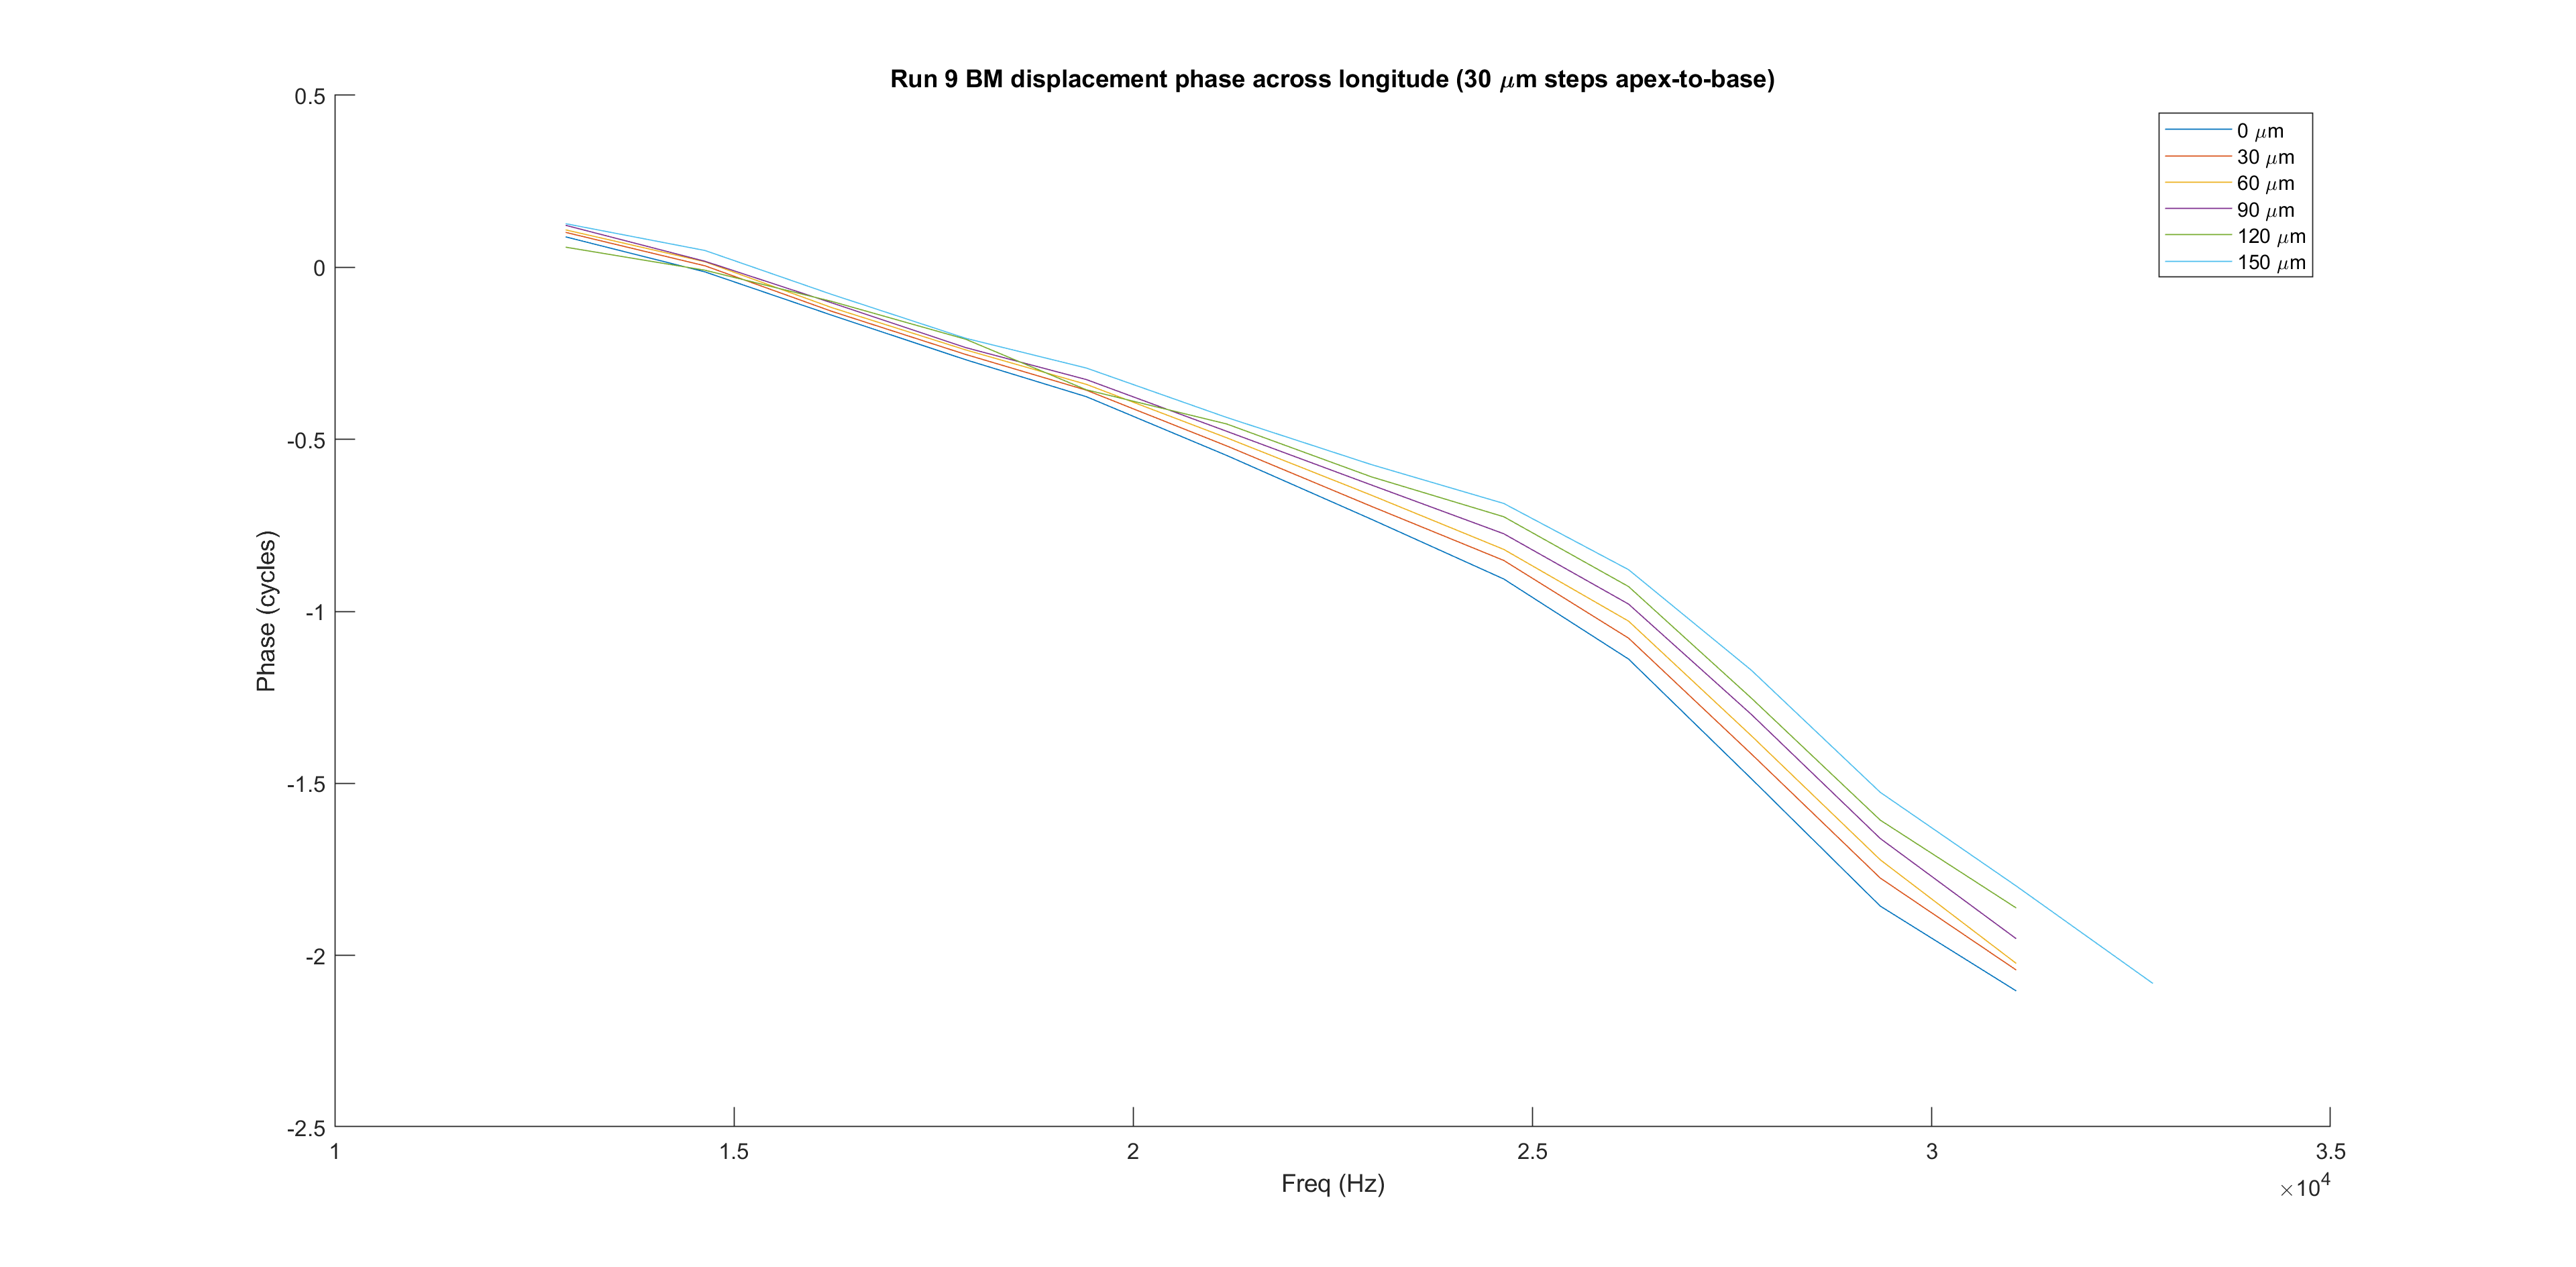
\includegraphics[width=\textwidth]{"Figures/Run 9 BM displacement across l.png"}
	\caption{BM displacement phase re ear canal pressures at different longitudinal positions. 11 positions spaced 15 $\mu$m apart longitudinally were measured in run 9, at a 45 degree angle from the BM normal. Every other position's BM displacement phase is shown, covering 150 $\mu$m of longitudinal space in the cochlea and showing the expected travelling wave behavior (more basal phases decay more slowly, as they reach their BF at a higher frequency).}
	\label{BMtravel}
\end{figure}

\subsection{Registration}
\par{ We make lists of the aligned BM and OHC points at both angles. We then register BM positions between the two sets of measurements. Because we don't know the absolute positions at which we are measuring \text{a priori}, we are not guaranteed that each measured BM position at one angle will match with a position at the other. In this example, we were able to match five positions corresponding to the most basal positions in run 9. Recall that this registration is performed via matching BM phases at either angle. These matching phases are seen in Figure \ref{BMmatch}.}
\begin{figure}
	\centering
	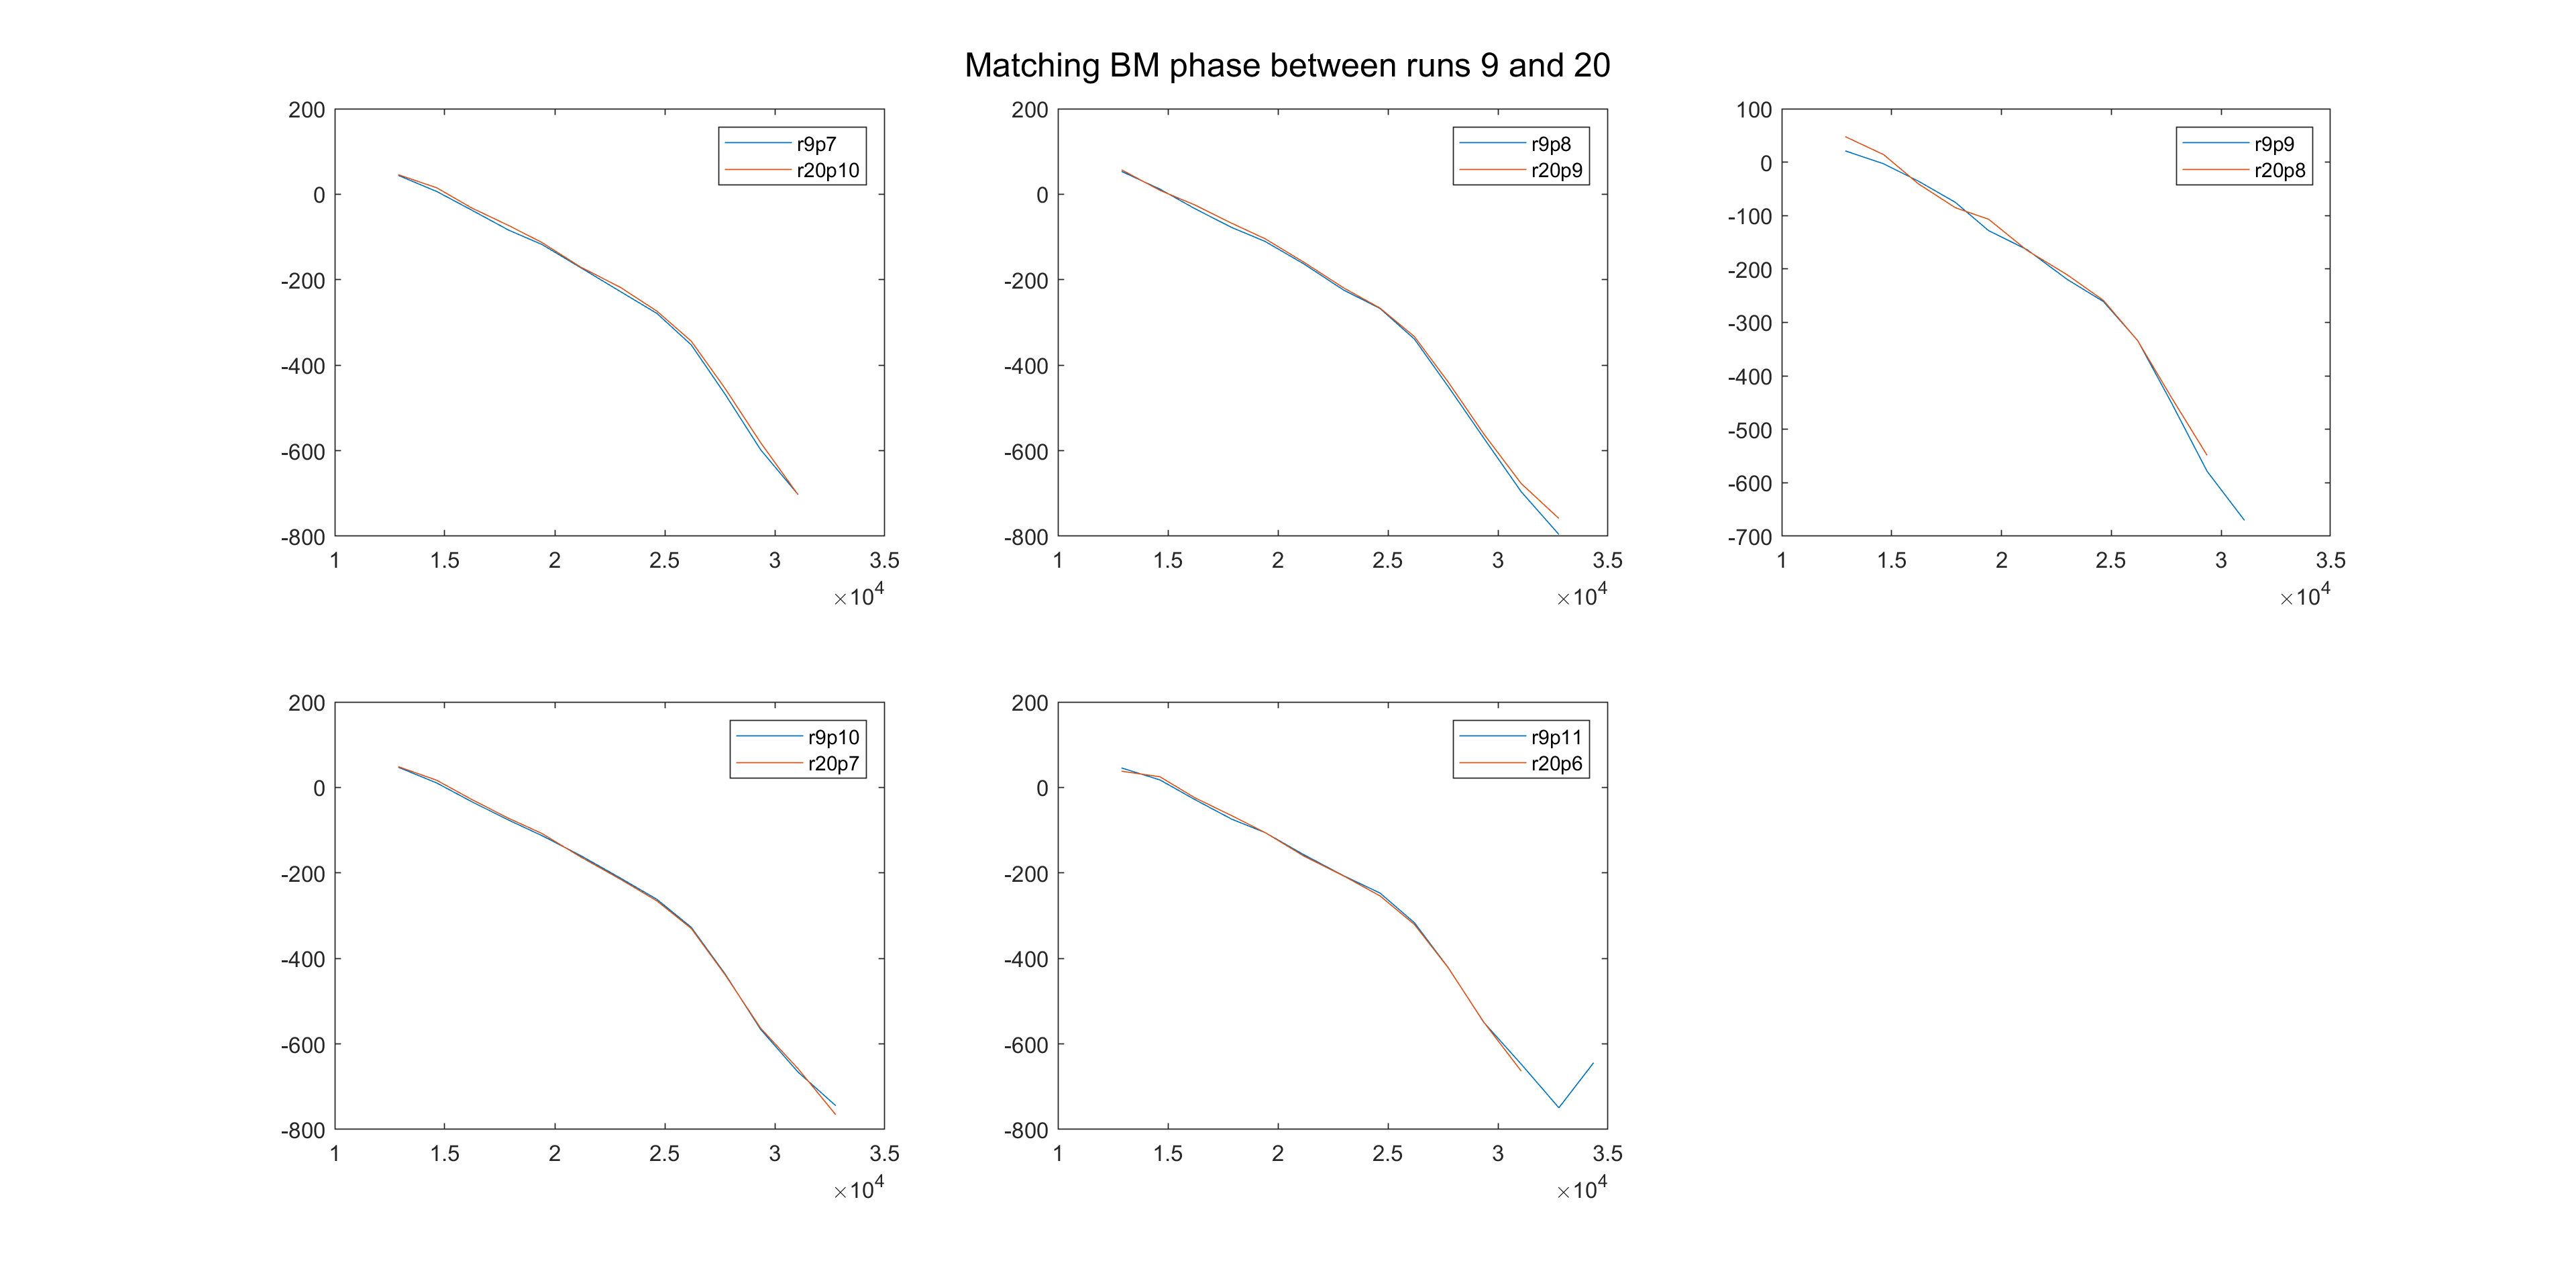
\includegraphics[width=\textwidth]{"Figures/Aligning BM9 and BM20.png"}
	\caption{Matching BM phases re ear canal pressure from five positions taken at both 45 and 60 degree angles from the BM normal. The points are 15 $\mu$m from one another, so these points cover a 60 $\mu$m longitudinal range of the cochlea.}
	\label{BMmatch}
\end{figure}
\par{Although it may not be completely obvious, the matched phases in Figure \ref{BMmatch} also provide evidence that our method is working as intended. Consider the match between points at Run 9 Position 7 and Run 20 Position 10 in the first panel. If this point is a match, then as we step basal at both angles, we should continue to see a match at every position. In fact, this is what we see for all positions up to the most basal position in run 9! This means that our steps are uniform between measurement angles. (Note that in run 9 increasing position index corresponds to moving basal, while in run 20, decreasing position index corresponds to moving basal).}

\par{We now turn to the OHC base displacement phase for the corresponding aligned OHCs. If these are characteristically different despite matching BM displacement phase, then we are guaranteed a nontrivial reconstruction. Figure \ref{alignedohc} shows aligned OHC displacement phases at 45 and 60 degree measurement angles. The phase measured at a steeper angle shows a significant lead, especially at high frequencies, whereas at low frequencies they appear in-phase.}

\begin{figure}
	\centering
	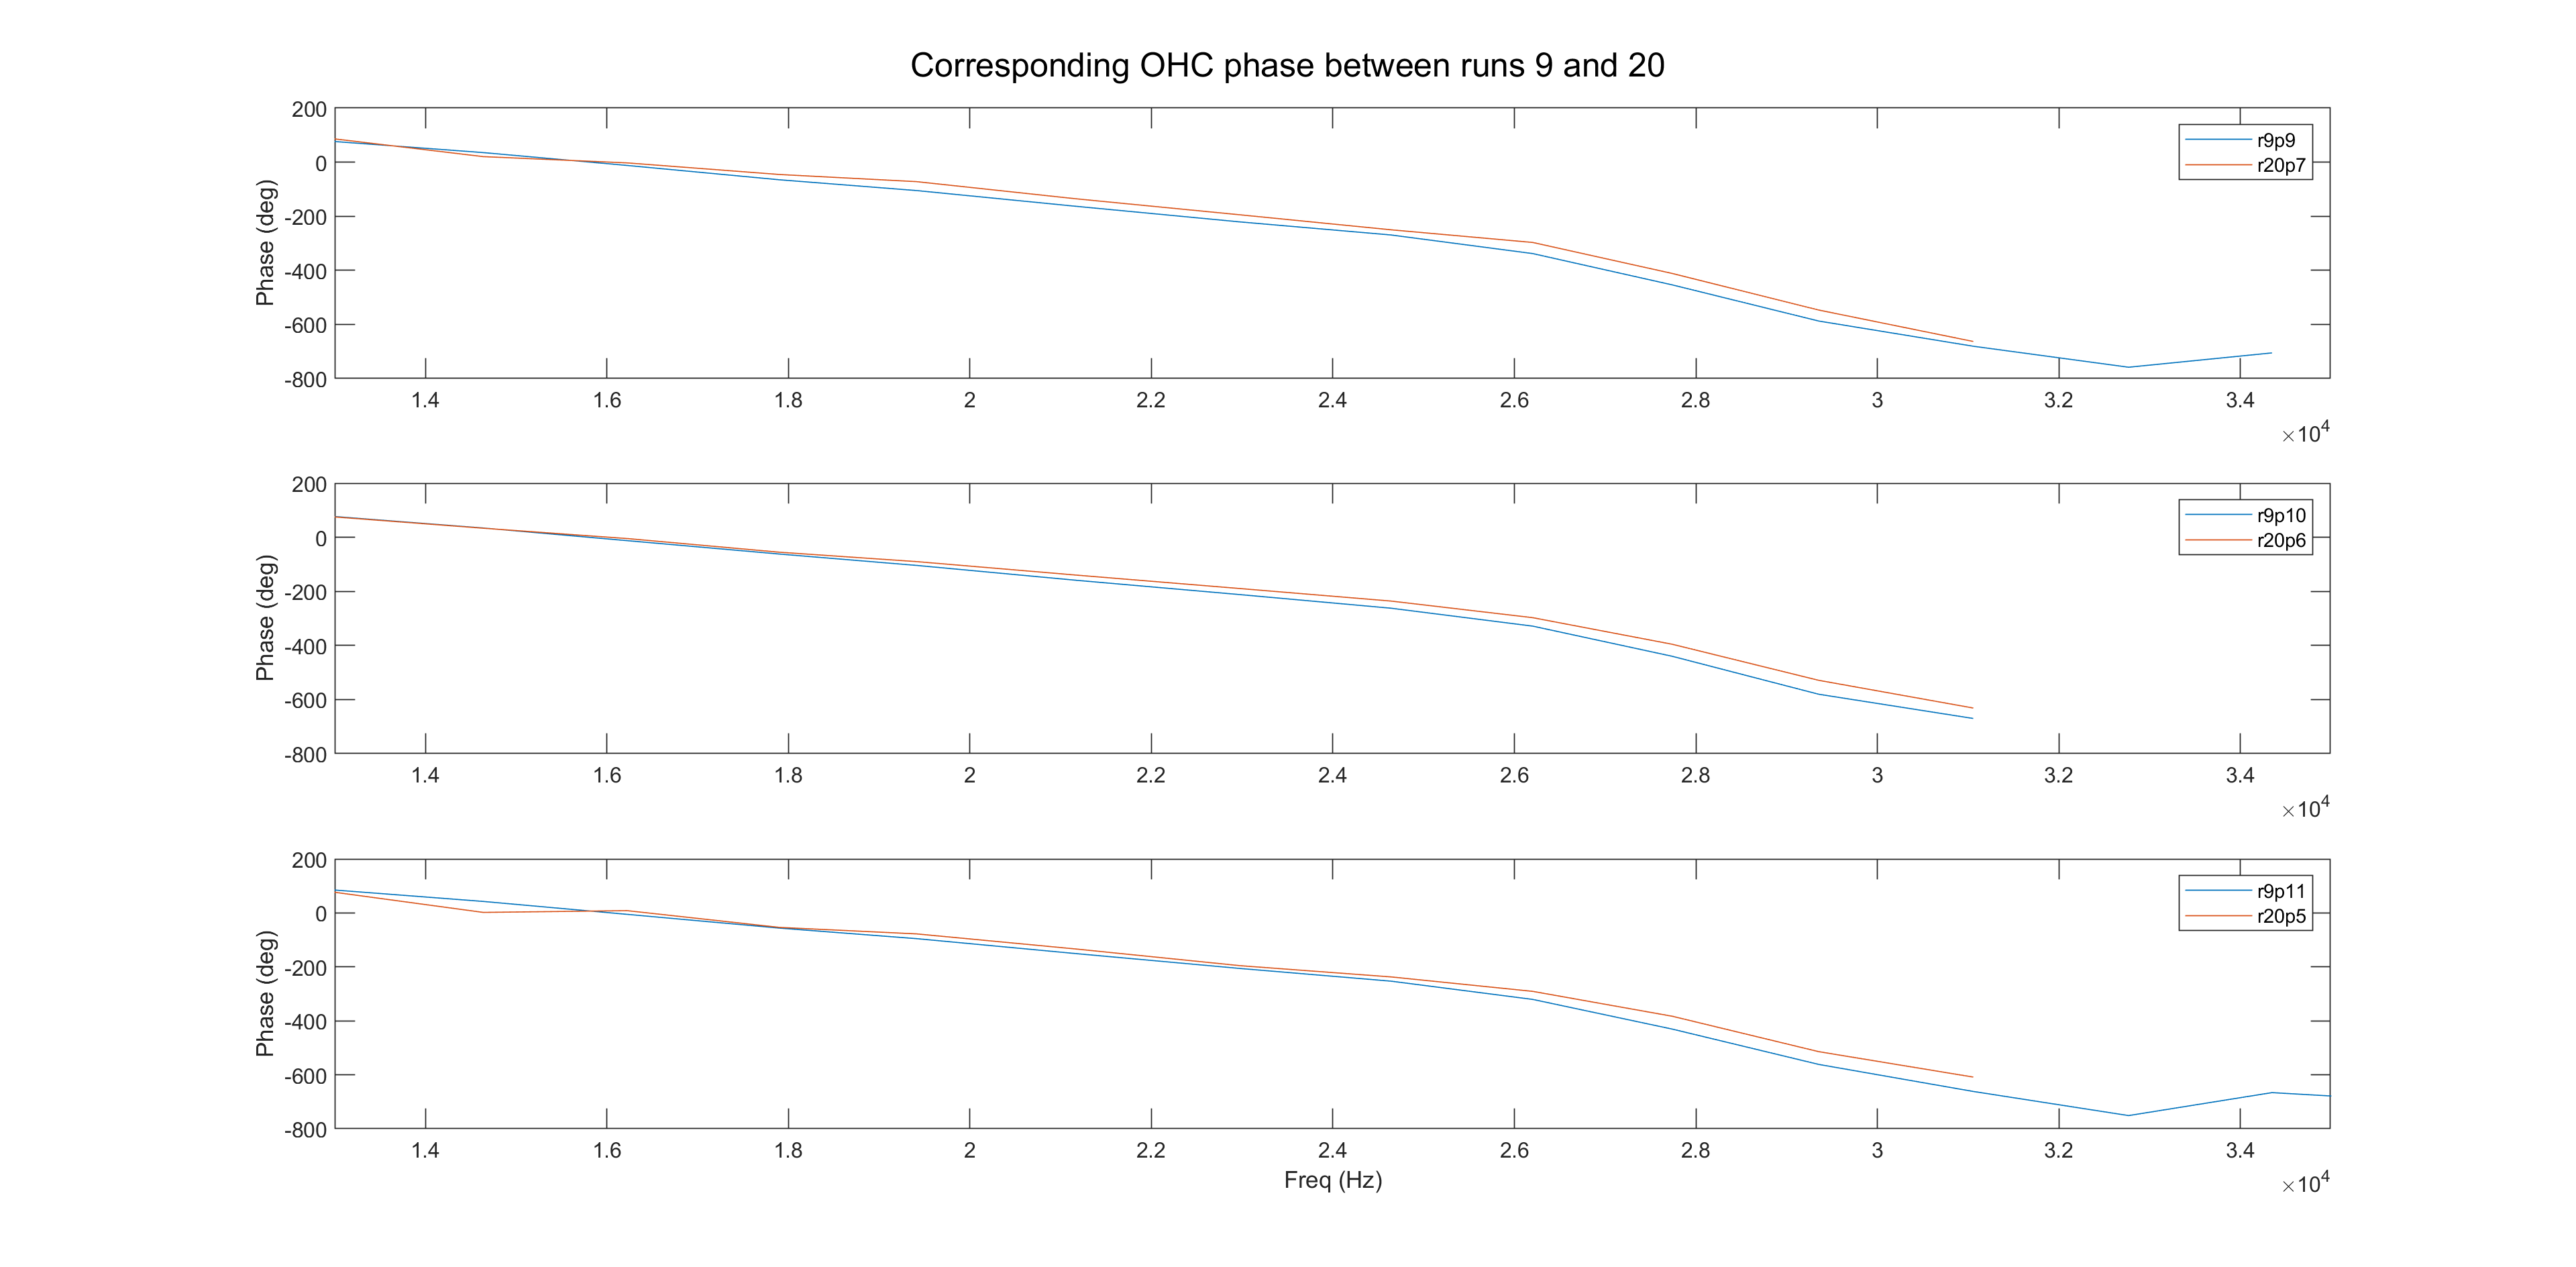
\includegraphics[width=\textwidth]{"Figures/Aligned OHC9 and OHC20.png"}
	\caption{Aligned OHC displacement phases at 45 (run 9) and 60 (run 20) degree measurement angles, and at 3 longitudinal positions. The OHC displacement measured at a steeper angle accumulates a lead over frequency with respect to the displacement measured at the shallower angle.}
	\label{alignedohc}
\end{figure}

\subsection{Reconstruction}
\par{At one of the points matched above, the measured BM in run 20 had no measured aligned OHC. For the remaining four matched points (along 45 $\mu$m of the cochlea), the reconstructed OHC transverse and longitudinal motion components are shown in Figures \ref{r8}, \ref{r9}, \ref{r10} and \ref{r11}. Here we have also displayed BM motion amplitude and phase, taken from run 9 where the angle of measurement is about 45 degrees. We have normalized the magnitude by multiplying it by $\sqrt{2}$, which is the geometric loss of measuring BM motion (which we assume is purely transverse) at this angle. We have not touched the phase.}

\begin{figure}
	\centering
	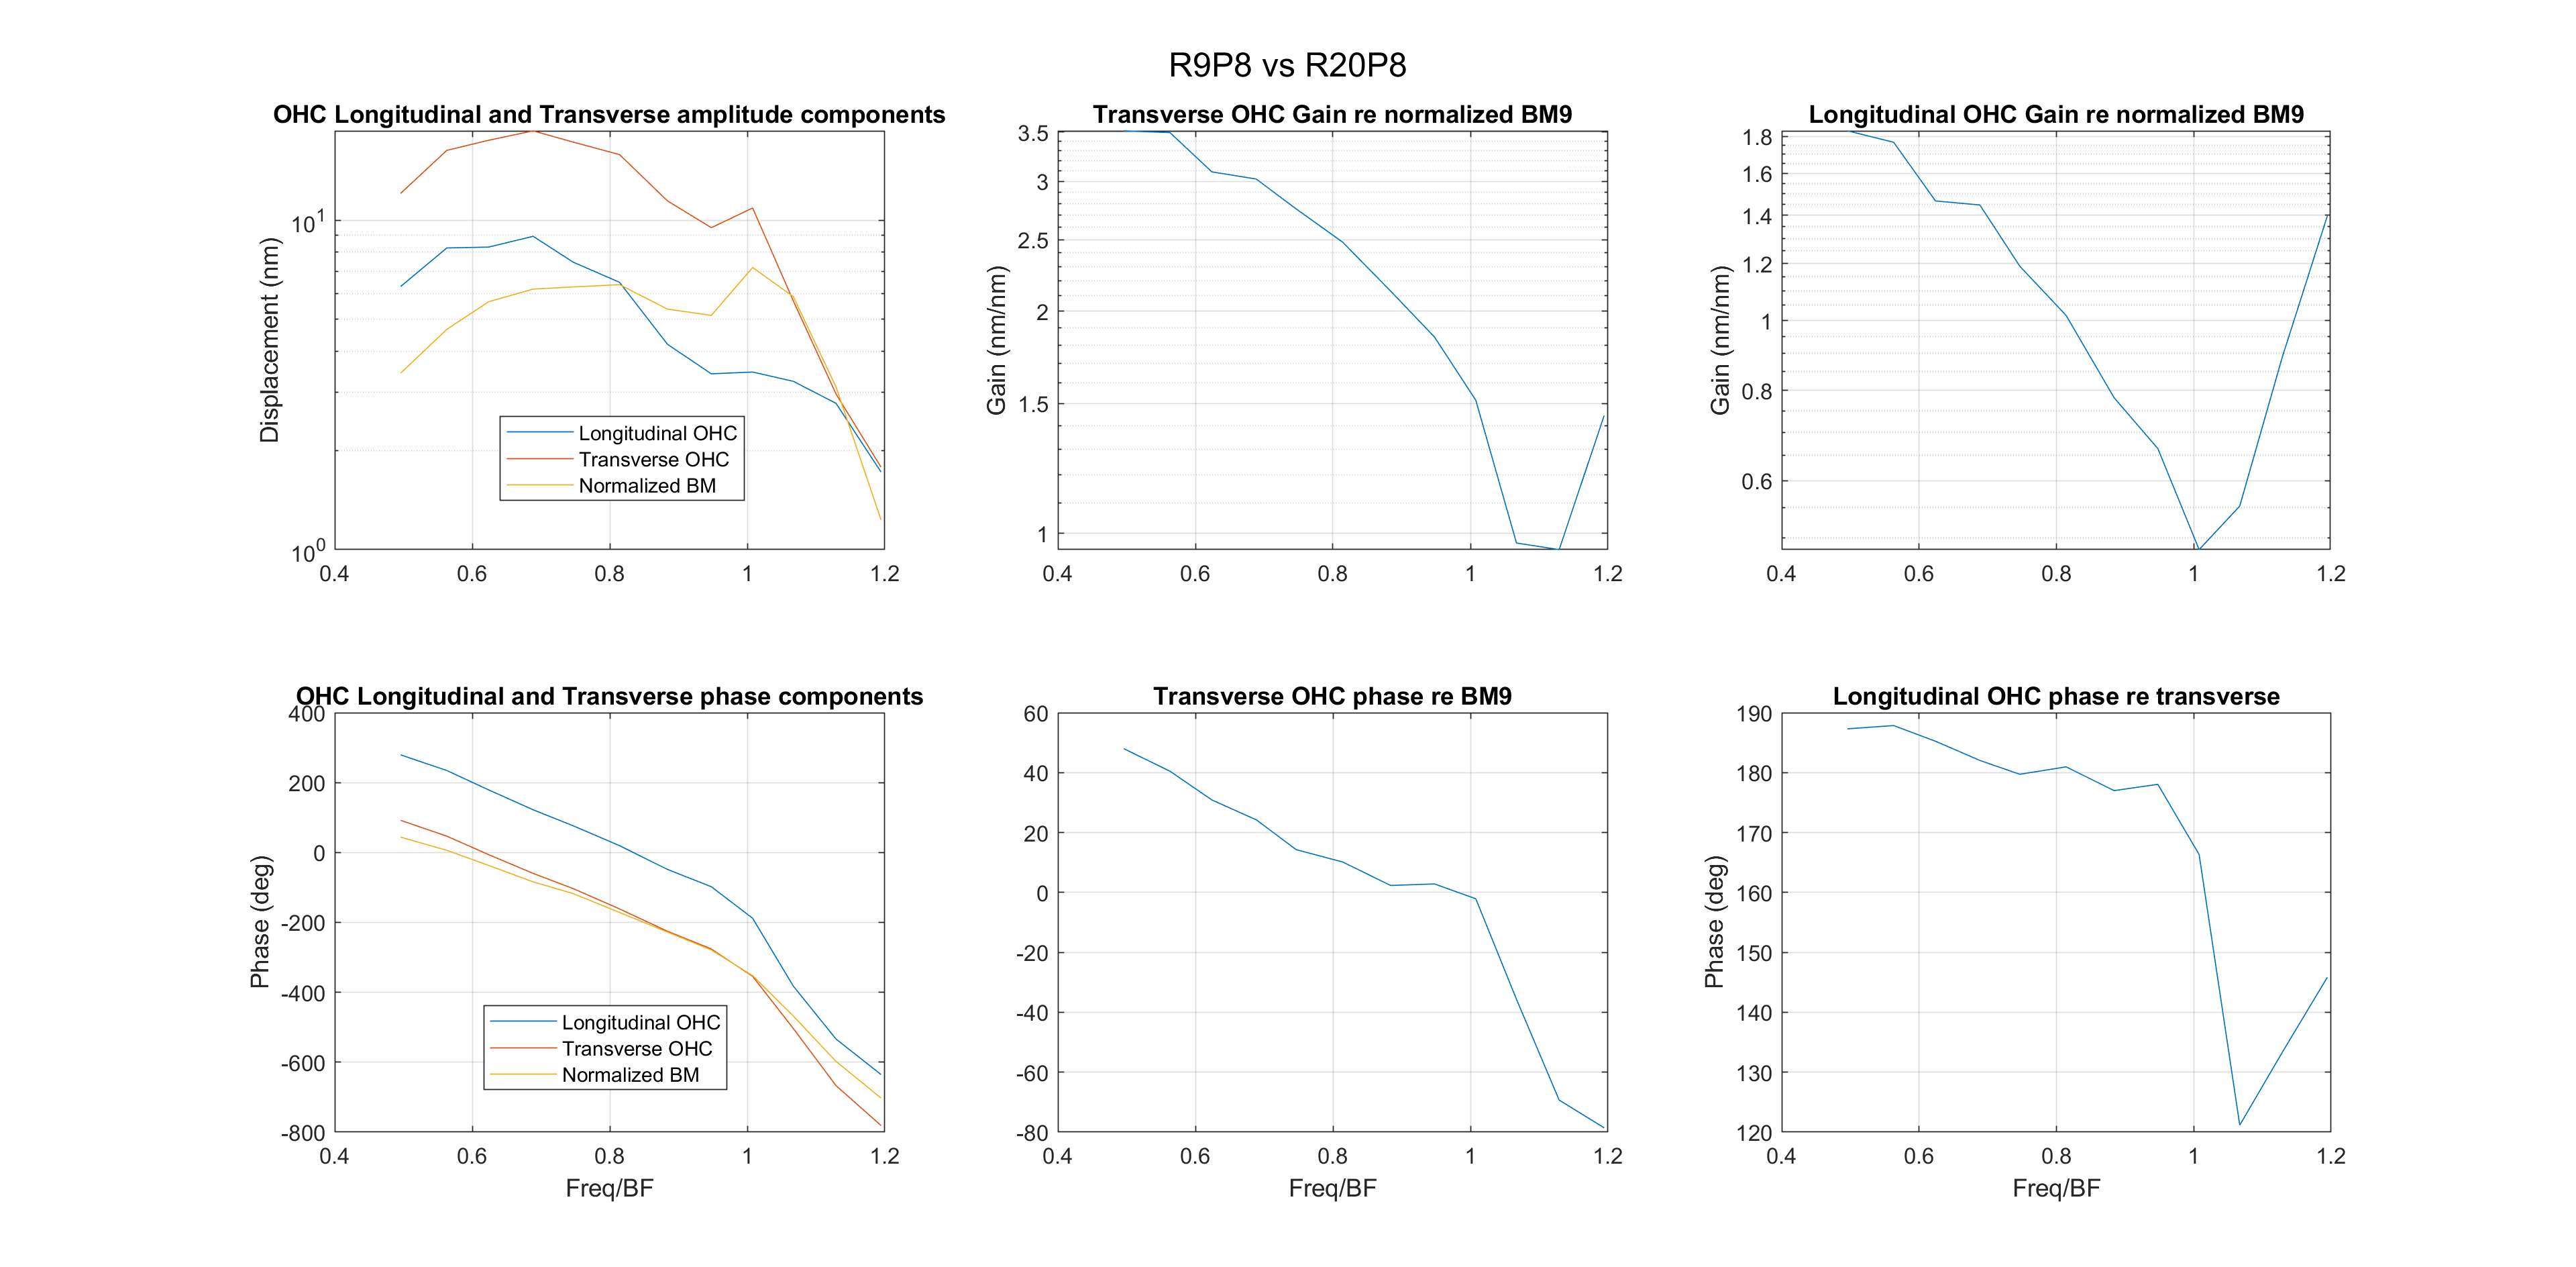
\includegraphics[width=\textwidth]{"Figures/R9P8OHC.png"}
	\caption{Reconstructed OHC base motion corresponding to Run 9 Position 8 and Run 20 Position 8, alongside run 9 BM motion amplified by a factor of $\sqrt{2}$. This is the most apical reconstructed OHC motion.}
	\label{r8}
\end{figure}
\begin{figure}
	\centering
	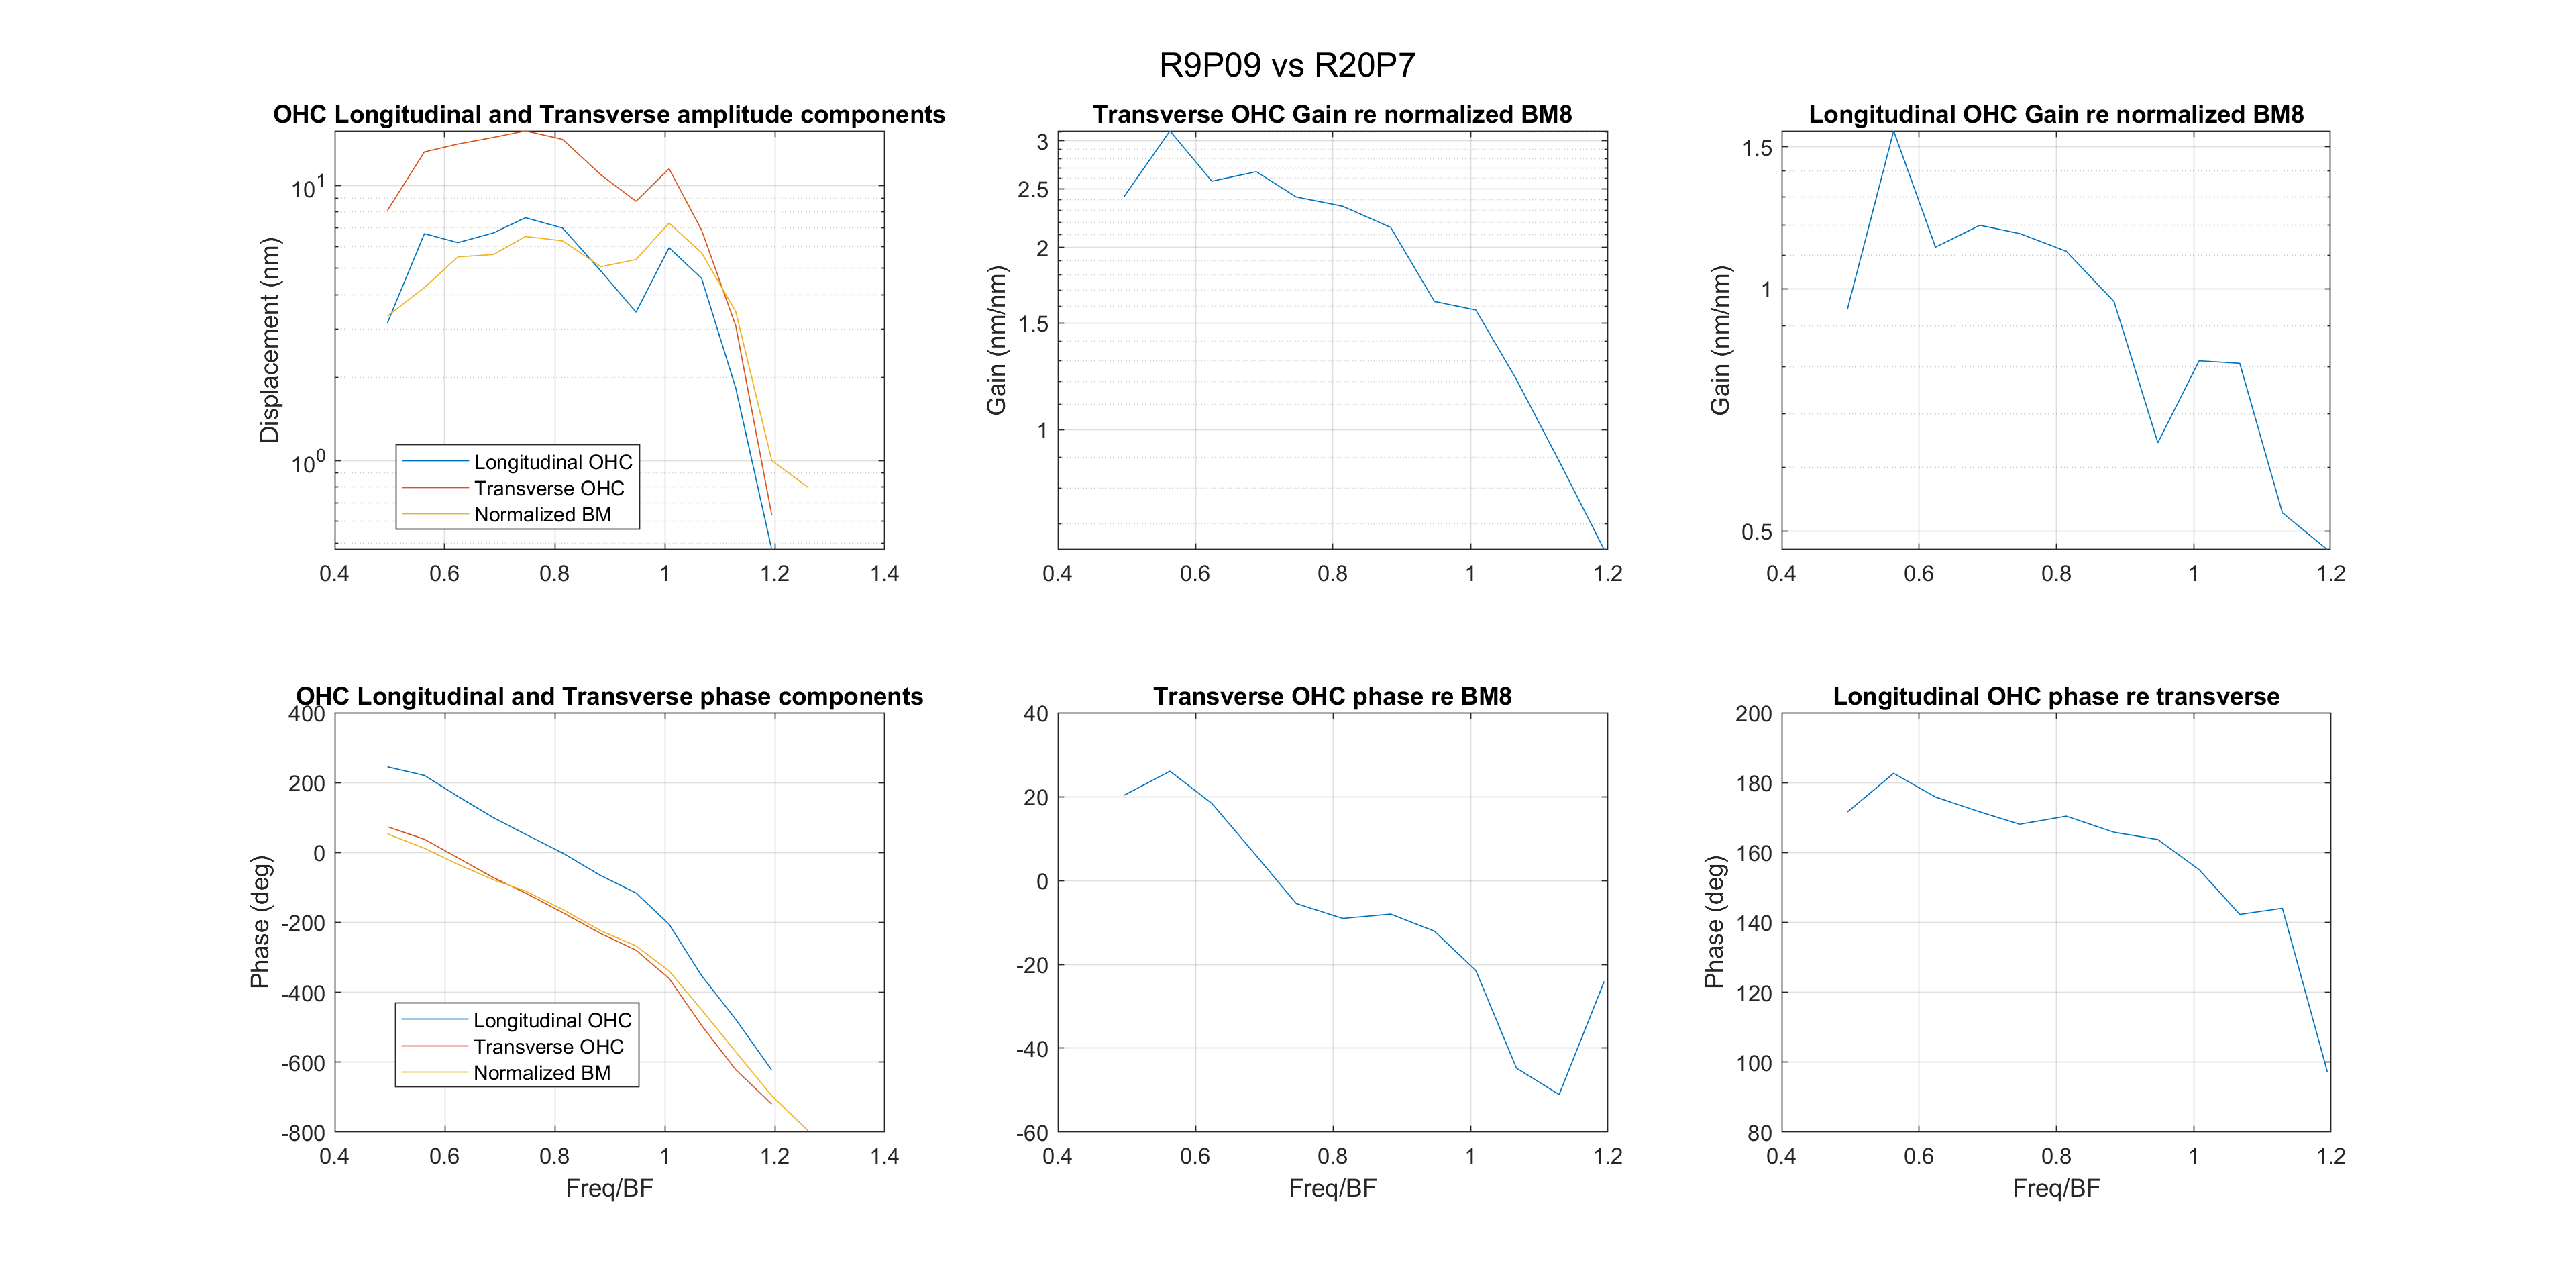
\includegraphics[width=\textwidth]{"Figures/R9P9OHC.png"}
	\caption{Reconstructed OHC base motion corresponding to Run 9 Position 9 and Run 20 Position 7, alongside run 9 BM motion amplified by a factor of $\sqrt{2}$. This is 15 $\mu$m basal of the OHC analyzed in Figure \ref{r8}.} 
	\label{r9}
\end{figure}
\begin{figure}
	\centering
	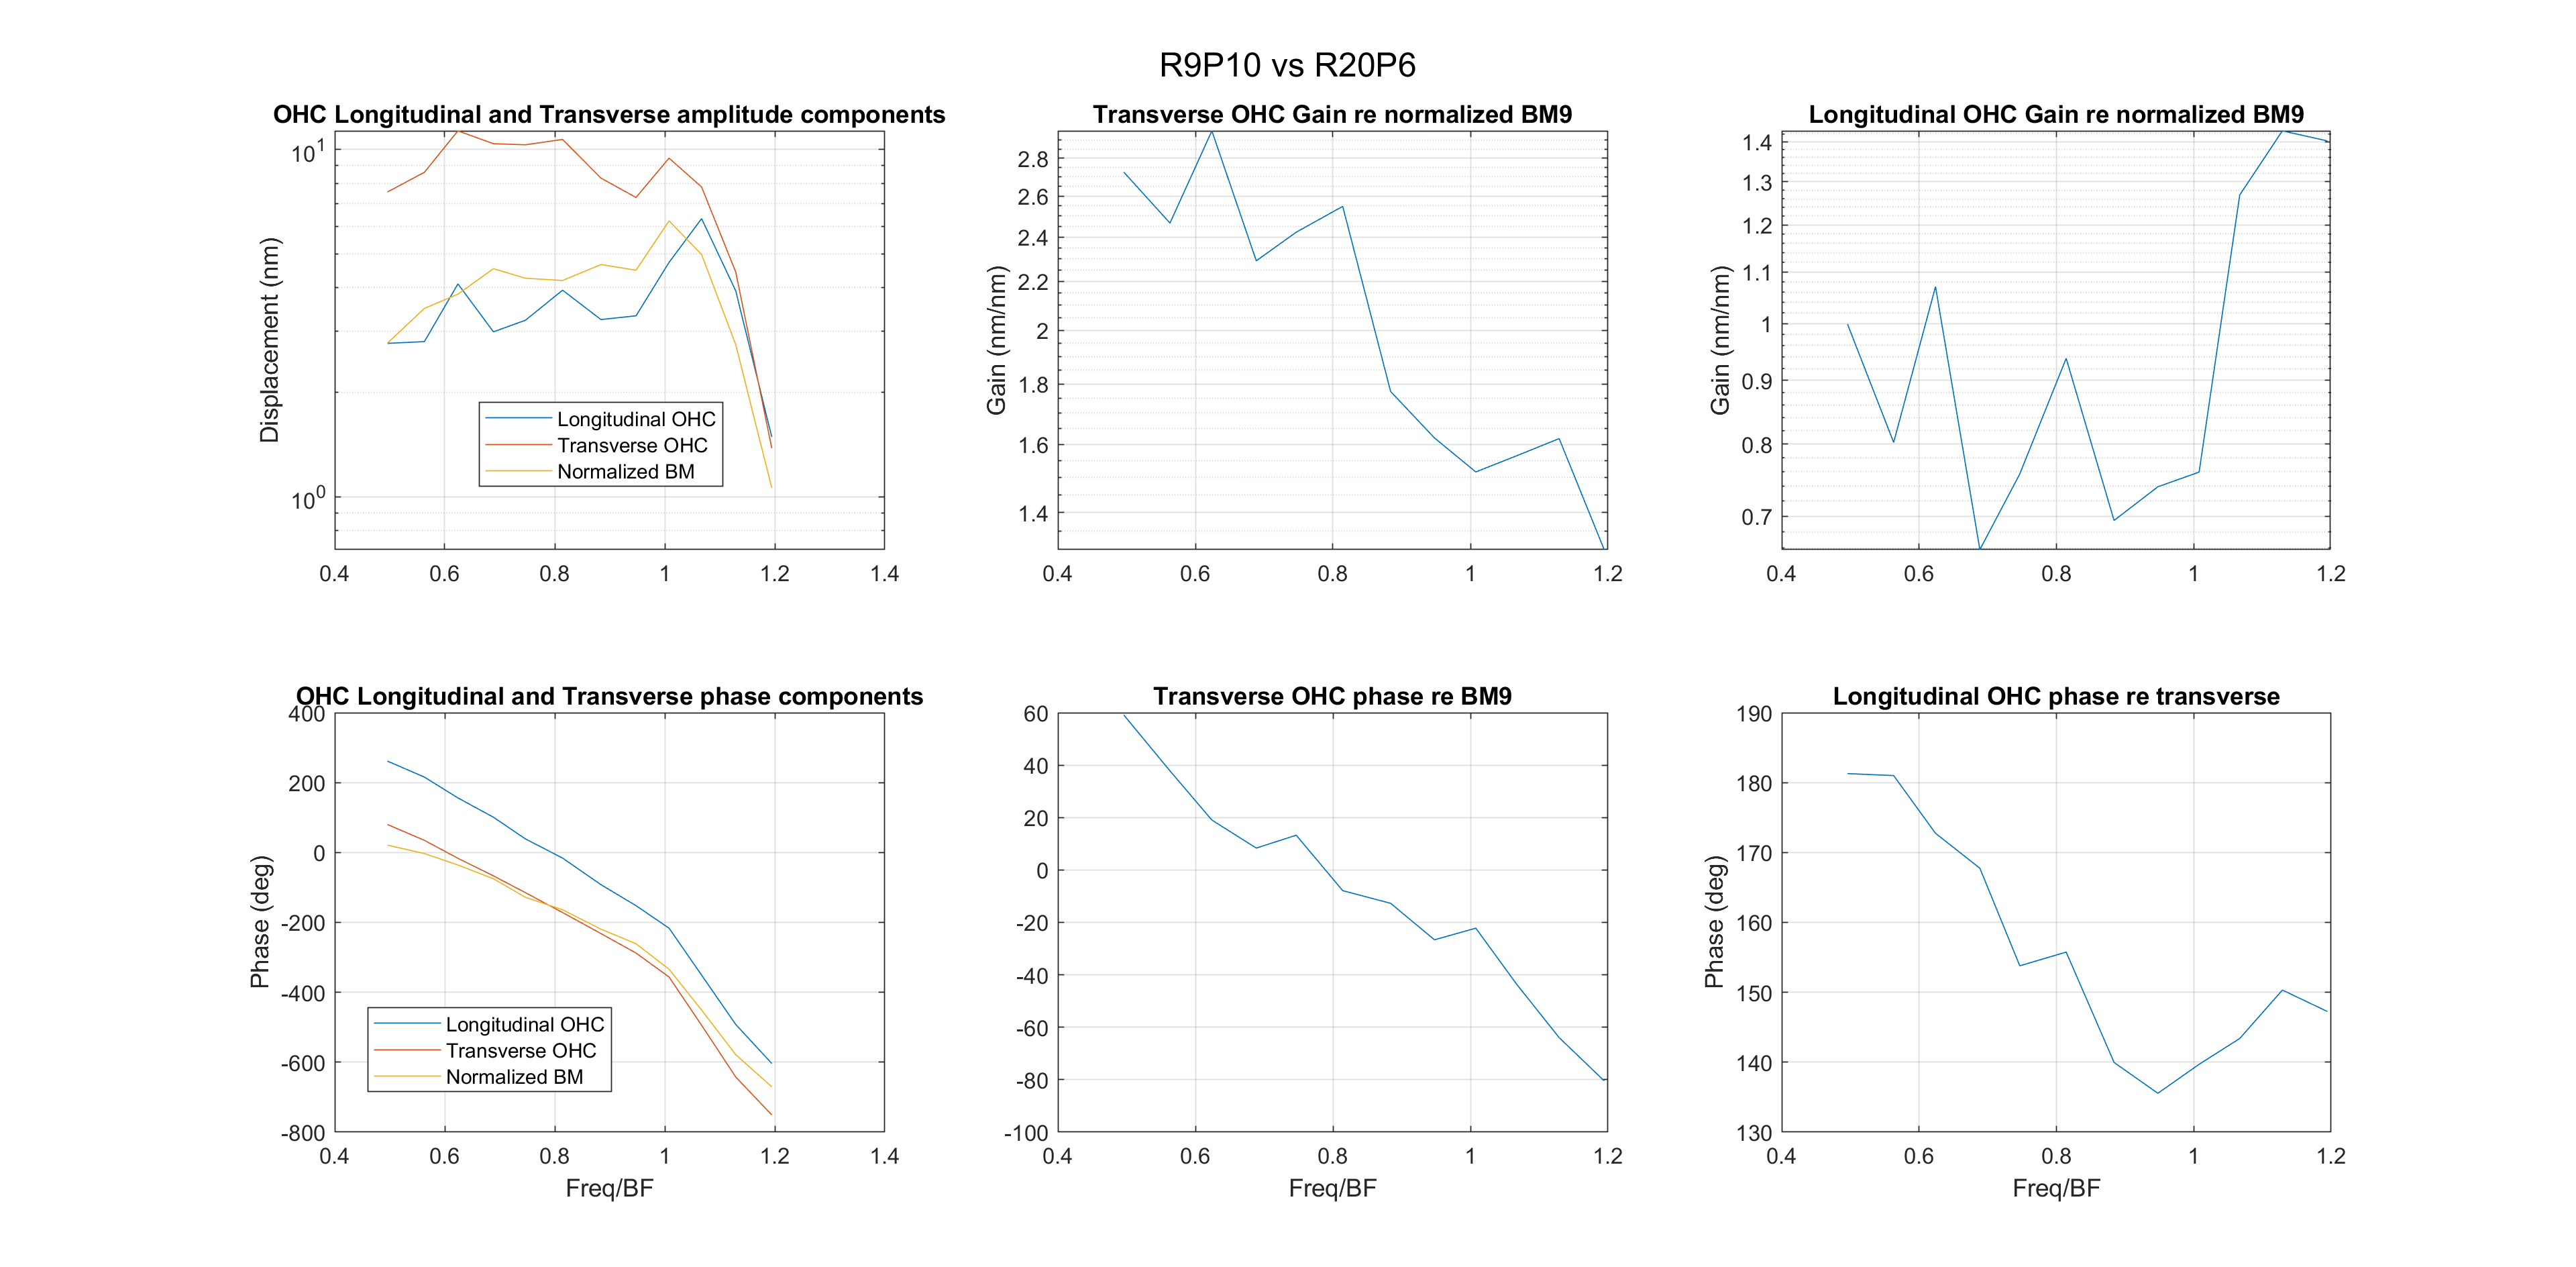
\includegraphics[width=\textwidth]{"Figures/R9P10OHC.png"}
	\caption{Reconstructed OHC base motion corresponding to Run 9 Position 10 and Run 20 Position 6, alongside run 9 BM motion amplified by a factor of $\sqrt{2}$. This is 30 $\mu$m basal of the OHC analyzed in Figure \ref{r8}.}
	\label{r10}
\end{figure}
\begin{figure}
	\centering
	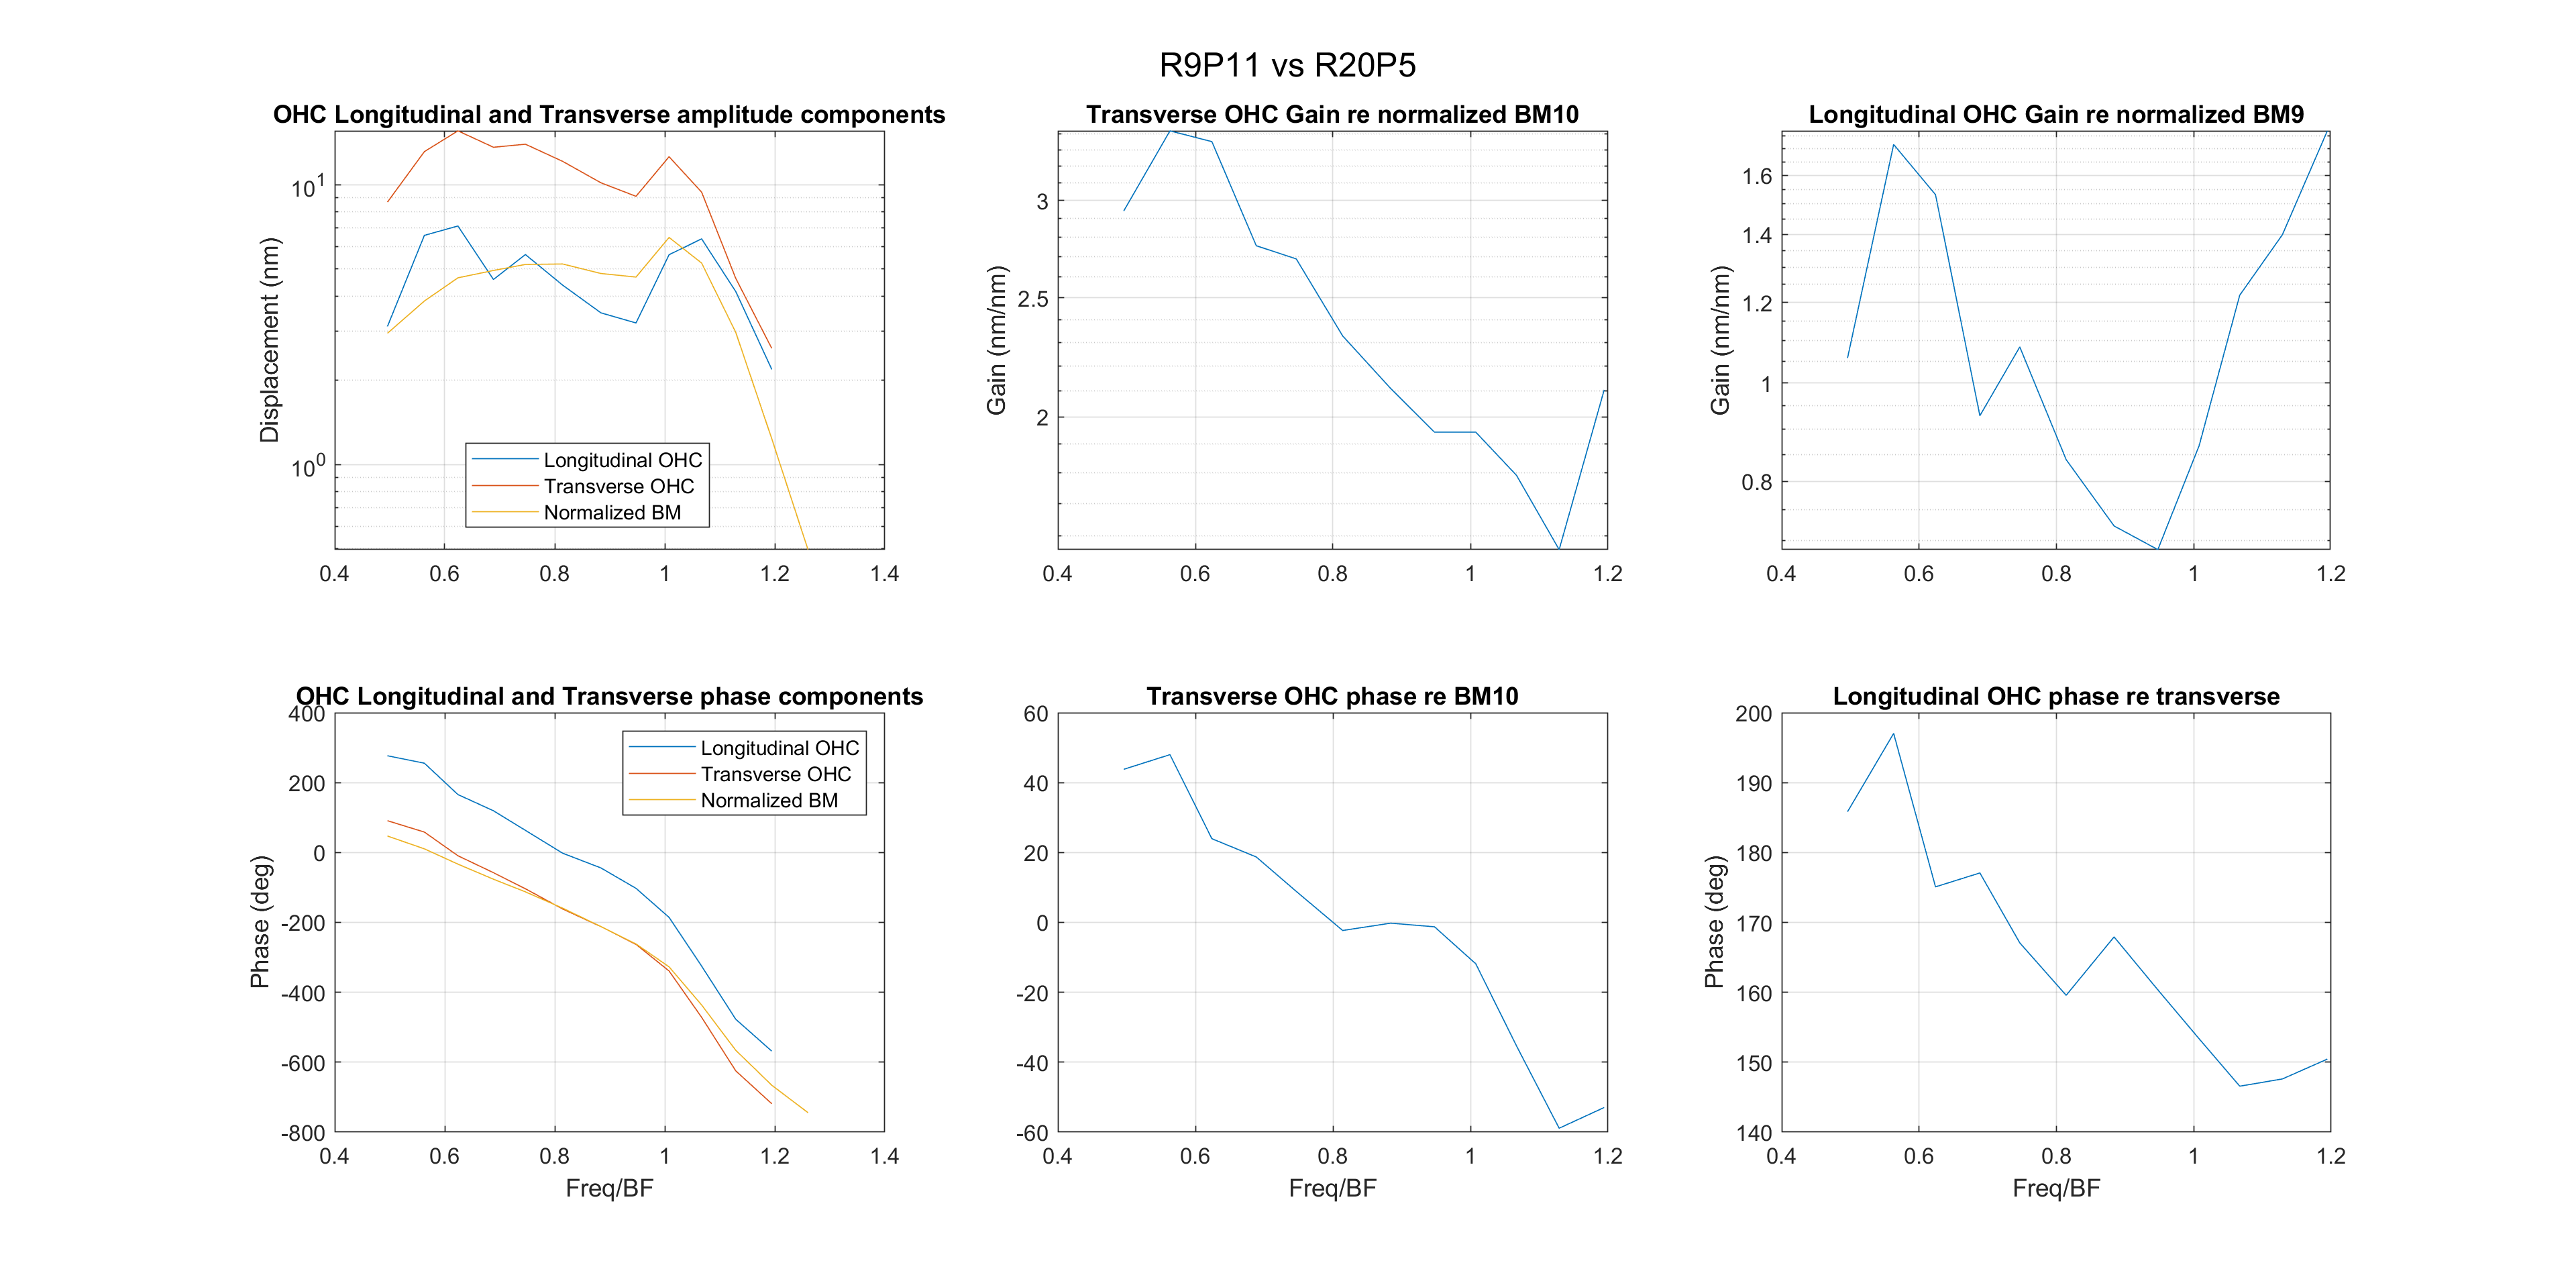
\includegraphics[width=\textwidth]{"Figures/R9P11OHC.png"}
	\caption{Reconstructed OHC base motion corresponding to Run 9 Position 11 and Run 20 Position 5, alongside run 9 BM motion amplified by a factor of $\sqrt{2}$. This is the most basal reconstructed OHC motion, 45 $\mu$m basal of the OHC analyzed in Figure \ref{r8}.}
	\label{r11}
\end{figure}

\par{While the curves here are not all ``beautiful," they share several characteristic similarities. Let's first consider the displacement, and recall that our condition number (about 8, as seen in Table \ref{kappas}) means our data is accure to about 0.8 nm. We see that both transverse and longitudinal motion share the low-pass qualities we see in our uniaxial OHC measurements at 80 dB SPL, but do both peak at BF alongside the BM. We see that sub-BF the longitudinal motion is significantly smaller than transverse motion, by a factor of about two, but this difference is smaller at higher frequencies. In magnitude, longitudinal motions seems more comparable to BM motion magnitude.}

\par{Perhaps more interesting is the phase, in which longitudinal and transverse components differ significantly. The transverse OHC base phase seems to lead the BM at low frequencies, but lag at higher frequencies. This accumulating lag corresponds to transverse OHC phase re BM decreasing monotonically in the shape of a (noisy) line. This line reaches zero around 0.8BF in all four of our reconstructions. In runs where high-frequency components were considered out of the noise, a lag of as large as 80 degrees was observed at about 1.2BF. While we didnt measure at frequencies below 0.5BF, we see leads of up to 60 degrees at 0.5BF.} 
\par{In the introduction, we discussed the work of Tianying Ren's group, and the disagreement between our phase data and theirs. This reconstruction is consistent with the data of Ren's group, as their measurements at what they note as a purely transverse angle also show this linear accumulating lag of OHC re BM. They see a lead of over 90 degrees sub-BF decreasing to a lag of about 80 degrees supra-BF, with the 0 crossing being around 0.8BF! This correspondence with their measured data both provides evidence that our method is functioning as intended.}
\par{The longitudinal phase is more elusive, as no group could hope to measure purely longitudinal motion. As longitudinal OHC displacements are smaller than transverse displacements, it is less represented in data taken at angles of around 45 degrees. However, our reconstruction shows an interesting character for the longitudinal phase that also seems to decrease monotonically as frequency increases. At lower frequencies, it is almost entirely out of phase with the transverse displacement, and this 180 degree ``lead" decreases to ~160 degrees near the BF. Where the phase offset is about 180 degrees, it means that the OHCs are moving in an angled linear fashion, moving towards the BM transversely in phase with an apical longitudinal motion.}
\subsection{Building intuition by working backwards}
\par{Here we have accounted both for the angle of projection and the relative positions of BM and OHC. We can make sense of our usual measurements by recalling the effects of each of these effects one at a time.}
\par{First, let's recall the case in which we only accounted for position. This is the case covered in \href{https://asa.scitation.org/doi/full/10.1121/10.0009576}{Frost et al, 2022}, Figure 6. Here, we saw that when we accounted for longitudinal position, OHCs always lead BM in the same cross-section by 45 to 90 degrees. This lead is largest at lower sub-BF and higher supra-BF frequencies. This data was measured at an angle of about 60 degrees with the BM.}
\par{We look at our reconstructed 2-D data on frequency regime at a time: at low frequencies, the dominating transverse components induce a lead, as seen in the graph, which decreases as we approach the BF; at frequencies near the BF, the dominating transverse component is nearly in phase with the BM, and the leading longitudinal component will contribute as well causing a slight lead in sum; at high frequencies, the transverse component actually \textit{lags} BM, but the longitudinal component's strong lead is now weighted more, as at high frequencies the magnitudes of longitudinal and transverse components are comparable. This explains the spatially resolved projected motion.}
\par{In our usual measurements, we see a different sort of pattern where OHC phase leads only at low frequencies, then is in-phase with BM at higher frequencies. This difference is displayed in the same figure from \href{https://asa.scitation.org/doi/full/10.1121/10.0009576}{Frost et al, 2022}. This is caused entirely by the travelling wave-induced phase difference.}

\section{Conclusion}
\par{We have developed a method to acquire data at points along the longitudinal axis with known longitudinal displacement steps. We have provided evidence that this method is functioning as desired by observing the expected travelling wave character of the BM displacement phase as a function of longitudinal displacement (Figure \ref{BMtravel}), as well as by showing the uniformity of the longitudinal steps across measurements at different angles (Figure \ref{BMmatch}).}
\par{We have employed our method for spatially resolving OHC and BM in the same cross-section to create pairs of aligned BMs and OHCs at different measurement angles. We have developed a physiologically motivated method for registering measured BM positions taken at different angles by matching their phase responses (Figure \ref{BMmatch}). This in turn allows us to register OHCs to one another, as they are associated with aligned BMs at each angle.}
\par{We have developed a simple mathematical method for using reconstructing the 2-D transverse-longitudinal motion of the base of OHCs from the 1-D measurements of the same registered structure at two angles (Equation \ref{fullreconstruct}. We have computed the effect that the angular difference between measurements has on displacement error (Table \ref{kappas}). We have demonstrated the application of this method \text{in vivo} at four longitudinal locations in the gerbil base (Figures \ref{r8}, \ref{r9}, \ref{r10}, \ref{r11}).}
\par{This preliminary data shows that transverse OHC base phase accumulates a phase lag re BM in a linear fashion, leading BM at low frequencies, being in phase with BM around 0.8BF, and lagging BM thereafter. These measurements are consisten with the transverse measurements made by the group of Tianying Ren.}
\par{The data also show that longitudinal OHC base motion is about half as large as the transverse motion in magnitude at 80 dB. It is also about 180 degrees out of phase (with respect to our coordinate system) with the transverse component of motion from low frequencies to ~BF, then leads by about 140-150 degrees at higher frequencies. This data suggests an approximately linear motion of the OHC base, with transverse towards-BM motion being in-phase with base-to-apex longitudinal motion.}
\par{We hope to collect more data of this type in the future, including data from the RL rather than only the base of the OHCs. We also were limited to using one SPL on account of the time taken per measurement and the phenomenon of drift in these experiments. Drift on the order of only a few microns can move a point measured from being right at the RL to being too far medial to get any OHC measurement, or from being at the OHC base to being too far lateral. This was accounted for in this experiment by taking data at one SPL so as to speed up the measurement process, allowing less time for fluid to accumulate on the round window membrane (the main cause of drift in our experiments.}
\par{If we continue to use the current method, it is important that we can control this drift in future. We would like to be able to ensure that we are measuring points at certain structures before taking measurements, and we would also like to not be limited to one SPL. One possible method is to place a cover slip on the round window membrane, which could eliminate the effect of accumulating fluid. We will try this in the next experiment.}
\par{Further into the future, I propose that we use a more robust spatial registration method (specifically the SIFT algorithm), which will greatly reduce the workload at acquisition time. Currently, we must take measurements over a reasonably short period of time, so we cannot simply take measurements at 200 points densely spaced across the cochlea at three different angles and hope to reconstruct motion. Moreover, over a larger space within the cochlea, the planar approximation inherent to our current method breaks down. With an algorithm like SIFT, we can track the volume over time and after each rotation, and spatially register points across runs under no assumptions about the geometry of the measured structures. I believe this will be necessary for densely-sampled reconstruction of 3-D intra-OCC motions.}

\end{document}
